%% Author: Jacob Osterhout

\documentclass[conference]{IEEEtran}
\usepackage{graphicx}
\graphicspath{ {images/} }

% correct bad hyphenation here
\hyphenation{op-tical net-works semi-conduc-tor}

\begin{document}

\title{Parallelized Game Tree Generation\\for Go}


\author{
\IEEEauthorblockN{Cindy Moline, Zachary Robertson, Jacob Osterhout}
\IEEEauthorblockA{Department of Electrical Engineering and Computer Science\\University of Central Florida, Orlando, Floirda 32816--8005}}

% make the title area
\maketitle


\begin{abstract}
Go is an exceedingly difficult game for an artificial intelligence to conquer; this is because generating a game tree is difficult, the branching factor is too large for most systems to handle. By splitting the work of generating a game tree, that could span all potential moves available at a particular moment in the game, among all the processors available to the system, we reduce the amount of time waiting for a move to occur. We believe that our implementation of the Randomized Best-First Minimax tree will perform legal game moves in a timely manner and will be able to make more effective moves by increasing the amount of utilized threads.
\end{abstract}

\section{Introduction}
The oriental game of Go is a two player, non-chance, combinatorial game with perfect information. So all of the information about the game state thus far is available to both players who take there turns knowing how their turn will affect the outcome of the game, each turn without exception contributes to the final score. On regulation sized 19 x 19 game boards there are 361 positions for game pieces to be placed. Each player has the option of placing a game piece, called a stone, or passing on their turn. The game ends when there are no available moves to be played or if each player passes on their turn in succession of one another. After a game is complete we enter the scoring phase, the winner will be chosen based on the number of opponent stones captured added to the total area on that board that is surrounded by your stones. Although the rules of Go are relatively simple, the dynamic nature of the game allows for much variation.\par
Each player, black and white, has an infinite amount of stones of that player's respective color. Black player will always be first to place a stone, the adjacent intersections are the most important positions on the board for a stone after it has been placed because they will determine whether that stone lives or dies. Each stone placed at the center of the board initially has four adjacent intersections which will decide the fate of the stone. Placement of a stone adjacent to one of your others' creates a group, this group has a greater number of adjacent intersections and is thus harder to capture. If stones of the opponents color occupy all of the adjacent intersections of your stone or group of stones than those stones are captured by the opponent and removed from the board. Since stones can be removed, placement of a new stone is forbidden if it recreates a previous board state, this rule prevents an infinite loop of capturing stones. Also suicide in Go is illegal, if placement of your stone would result in one or more stones of your color being removed then that move is not allowed.

\subsection{Complexity}
Each location on the board has only three potential states, empty, black or white. On a game board with N locations there are a total of $3^N$ possible board states. Tromp and Farneback showed that on a standard board only about 1.2\% of board positions are legal, using this fact we can estimate the number of legal board states for a 19 x 19 board as \[3^{361} * 0.012 = 2.08\dots * 10^{170}\]This number demonstrates the vast amount of variation inherent in Go, also that our game tree will obviously not be able to explore every possible variation of board combinations. Therefore if we choose to implement a standard game tree, we would need to optimize it with pruning and only expand those nodes which we feel will lead to a positive outcome. Standard alpha-beta pruning techniques identify moves that are so good for the current player that best-play by the opponent should not have allowed it. Another type of pruning very relevant to Go, due to the option to pass on your turn, is null-move pruning in which the computer imagines that it has given up its turn and imitates a shallow alpha-beta search. If this search results in a cut-off, then we do not need to expand this entire tree because we know it is now very likely that actually making a move also produces a cut-off.\par
Victor Allis notes that typical games between expert players last about 150 turns each with an average move complexity of 250 choices, we expect that our game tree will have a similar average branching factor. This means that each node in our game tree will have around 250 child nodes, with more initial children at the start of the game tree and very few children near the end. Games with a high branching factor make classic search algorithms like an unoptimized minimax search extremely costly.

\begin{figure}[h]
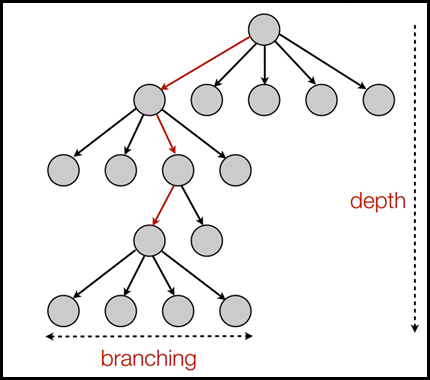
\includegraphics[width=200px]{branching}
\centering
\end{figure}

\subsection{Game Trees}
The traditional approach of combining alpha-beta search with a heuristic position evaluator is very difficult to do for the game of Go. Creation of an adequate static position evaluator is one of the main hurdles for writing an artificial player for Go. Even if we reduce the standard board size to 9 x 9, which in terms of complexity is inferior to Chess, the traditional minimax game tree approach does not create a strong player [4]. One of the only times the computer player is aware that a move is good is when the opponent is about to have some of their stones captured. Most of the strategic positions in Go are dynamic in nature which lends itself to the randomized branch selection inherent in a Monte-Carlo evaluation. Since Go is deterministic we can generate actions at random until a terminal board state is reached, some if not most of these random play-outs will result in a better outcome than trying to abide by a heuristic that leads to predictable play.\par
Monte-Carlo Tree Search (MCTS) can be used in any combinatorial game and is based on many play-outs, the final game result of each play-out is then used to weigh the nodes in the game tree so that those nodes which lead to more favourable results are chosen during actual game play. It combines the generality of random simulation with the precision of a tree search. It does not require any strategic knowledge of the game, just its legal moves and ending conditions. Games with a large branching factor are suitable for a Monte-Carlo search because they have much less space complexity than a breadth or depth first approach, since MCTS does not attempt to expand every leaf of the game tree. Due to the random nature of the algorithm there are situations where finding a reasonable move is difficult, as the vital nodes may not have been visited enough times to give desirable results. This kind of search can be quite time consuming as many nodes must be expanded in order to produce strategic moves, techniques such as parallelism and conjunction with domain specific knowledge can significantly improve the speed.
\subsection{Parallelization}
In order to obtain parallelization in a search algorithm, speculation must be used. In a normal serial game search algorithm the next node to search is chosen when the previous nodes finish there evaluation. So we finish evaluating all a node and then evaluate the tree.  At this point the children of the last node chosen will have the most up to date scores and we choose the best to evaluate first. The problem is this has no parallelization. In order to have parallelization we have to start evaluating nodes before the previous nodes are finished. This is speculation.\par
There are two types of speculation fine grained and coarse grained. Coarse grained speculation allows the search space to be very large while fine grained makes it small. Coarse grain will do a lot of extra work. It searches a lot of places where the search really doesn't need to be done, but because we have processors available it likes to keep them busy. For example a coarse grain approach will search through a node that has already been evaluated as being no good just to keep a processor busy. If we try to resolve this issue, then we can encounter a scenario where the approach is too conservative about which node to speculate on, resulting in idle threads.\par
Instead, RBFM uses a fine-grained approach. For each processor we have that processor process a node. When that processor is done expanding a node it will update the shared tree structure so that when the next node is expanded it will have updated values to when choosing the next node to expand. This makes the speculation fine grained. But updating the tree we are able to remove nodes that would be useless extra work for one of the processor. Each of the processors does not care what the other processors are doing. This avoids the problem of global synchronization. Each processor will expand its node, do its thing, and start over. There is a synchronization point when need to worry about.  When two processors are trying update the same node. In this case locks are used to ensure mutual exclusion. The structure of the tree does not change only the scores of each node. The tree only grows so only one node needs to be locked at a time. The authors believe that their approach produces high quality speculations, and we agree. By running threads concurrently, this should not affect the value of a leaf node when it gets expanded. Instead, the speed at which iterations occur should increase. 

\section{Implementation}
Since we are well aware of the computational difficulty inherent in games where the sheer number of potential moves can overwhelm an artificial intelligence's ability to determine the correct course of action, it follows that the more nodes we are able to compute in a time-frame that humans find reasonable to take a turn in a game, then the more accurate our program will be at playing said game. This is why the next step in developing an artificial intelligence that is proficient at the game of Go is dependent on the processing power of the computer running the artificial intelligence software. Expanding our game tree concurrently will allow us to explore more nodes than we could in in same time sequentially, ideally with a lock-free implementation we would expect a speed-up equal to the number of threads that our implementation has availability to. This speed-up will obviously not be achieved as our solutions cannot completely run concurrently, instead they will implement various locks as needed to ensure that redundant work is not done and data integrity is upheld. Both of our chosen implementations have best-first search methodology, which means we will not actively try to expand all nodes but instead choose nodes to expand based upon some reasoning. Traditional game theory suggests that most games should be winnable using a minimax tree, although we understand the difficulty of the implementation in Go, with a high level of parallelization we believe that our implementation can overcome the difficulty of intermediate evaluation and produce a bot that exhibits strategic game play throughout the game with little to no possibility of skipping the most desirable move at a specific board position. As noted by Chaslot, Winands and Jaap van den Herik, currently a Monte-Carlo tree search program named \textit{Crazy Stone} holds the highest rating amongst all the other programs recognized on a particular Go site as well as won the second Computer Go University of Electro-Communications cup, since this implementation is state-of-the-art it seems important for us to parallelize it as well.\par
Other implementations of Go playing artificial intelligences include algorithms that employ machine learning or are knowledge-based systems. Both of these other strategies rely on examining the results of many previously played games and matching the currently executing game board configuration with those results which ended with a positive outcome. These algorithms require significant time and effort to implement and do not lend themselves as easily to the parallelizable nature of game trees. Also our implementation is relatively lightweight in comparison with these alternatives, with most of the computation occurring during the execution of a game.

\subsection{Monte-Carlo}
Research indicated that there were several different valid techniques for accomplishing concurrency. All of these stemmed from the same four steps which are the basis of a MCTS implementation. The first of which is \textit{selection}, during this phase a leaf node is chosen at random from the root of our game tree. Second is the \textit{expansion} phase which examines the leaf node chosen in step one and determines if it is represents a game board where the maximum number of moves has been reached. Assuming that the leaf node selected does not represent a completed game board, we proceed to the \textit{simulation} stage, where random plays occur until the maximum number of game moves have been played. Finally we score the board and take note of the wins and losses, during the \textit{backpropagation} step we update the corresponding nodes from the leaf node chosen in step one to the root of our game tree.

\begin{figure}[h]
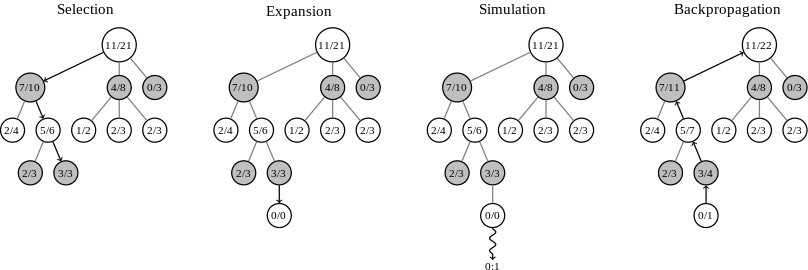
\includegraphics[width=235px]{MCTS}
\caption{Steps in the MCTS algorithm}
\centering
\end{figure}

Our implementation of a Monte-Carlo Tree Search is mostly based off tree parallelization. This method uses a shared game tree in which each thread is simultaneously playing a random game and expanding that specific branch of the game tree. In designing our implementation we had to consider whether to focus on exploration or exploitation.  If several threads start from the root of our game tree at the same time, there is a chance that they will traverse the tree in a similar fashion. Since heuristic values are hard to compute for intermediate game board states in Go, we decided to focus our design on exploration. Thus when a thread plays a game it only looks to explore nodes from the current root node's children only, once an expansion reaches a game board state with only one move left we explore all possible moves before propagating our wins and losses back to the root, this is our exploitation step and helps us to get a better idea of the destination's value. It is worth noting that since we explore all leaf nodes final scores we only need to lock the leaf node's parent in order to reduce redundant work done by other threads, thus terminal nodes will only be visited once by one thread. Since multiple threads will still have the potential to explore games from a specific child of the root node, we use atomic integers to represent the number of wins and losses for a node. After a time period of thirty seconds has passed, we will not continue to expand random child nodes, once all threads have terminated we look at the difference between the wins and losses for each child node and choose the one that is most fit. After a turn is complete our game tree trims all non-selected children and after the opponents move, will choose this node as the new root node.

\subsection{RBFM}
Our implementation of a parallel minimax tree search comes in the form of a Randomized Best-First Minimax Search (RBFM). Shoham and Toledo introduce this efficient selective search algorithm which attempts to focus on relevant nodes. RBFM associates a minimax value and a probability distribution to each node, when the algorithm expands a leaf node in the tree it updates the relative parent nodes minimax value. Each leaf is chosen based on a random walk from the root of the tree, given more precedence to those nodes with a higher probability distribution. The random nature of this algorithm creates parallelism since we can assign a different random walk to each processor. A regular best-first search would only expand a leaf node if it had the highest current heuristic; this introduces a problem as the initial best move does not always lead to a favorable outcome for the entire game. RBFM fixes this problem by expanding all children with some probability down to a specified depth.  This method of expanding nodes seems to fit the randomization that is preferable in Go as well as outperforming the alpha-beta method of selecting leaf nodes.\par
When the algorithm runs on a parallel computer, the amount of work is minimized because threads do not waste time waiting for a node to finish being evaluated. If each thread were to wait for the evaluation of any node, this would serialize the entire process. The only time when contention happens in RBFM is if two or more threads are attempting to update the value of a single node, once there are many nodes on the tree this becomes less of a concern. When a thread finishes expanding a node path it backs up the score and starts over again at the root, this way the processors remain busy.

\begin{figure}[h]
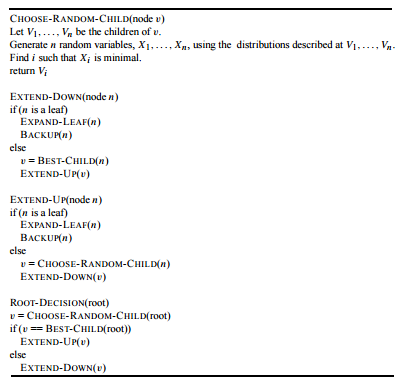
\includegraphics[width=235px]{RBFM}
\caption{Pseudo code for the RBFM algorithm}
\centering
\end{figure}

Our algorithm uses a shared-memory model in which all processes access a single search tree, these processes will lock nodes when they traverse the tree but since the tree only grows without transforming there may only need to be one active lock per process. Our primary motivation for this over the master-slave technique was primarily to avoid more complex code and faster computation. Although the speed difference may not have been that significant, we suspected that there would be some overhead in allowing all slave threads to send messages to the master. At which point, it would then have to search the tree to make the necessary update for each individual request. Shared memory model only becomes expensive in a distributed system, due to the extra time spent communicating tree updates between processor cashes. However, this is not the case for our testing machine.\par
Our approach iteratively expands a leaf node and propagates a score based upon a simple static board position evaluator, up to the root of the tree. There will be some cases where expanding a node and updating its minimax score cannot change the decision at the root; in this case RBFM avoids expanding these nodes. One thread of execution will always be exploring the moves that spawn from the best play but others will continue to search for moves in leaf nodes with less desirable initial results, in this way we are not guaranteed that our algorithm will always choose the greedy move.\par
Generally, iterative algorithms are highly parallelized, because each thread can sequentially run the sequence of steps and improve the approximation by multiple factors . So in the case of the RBFM, it would be deemed embarrassingly parallel, since each thread can essentially can run an iteration over the tree, therefore, improving the odds of game play faster than in a serialized process. During our expansion of nodes in parallel there the only time we need to lock a node is when it is currently being expanded by a thread. These locks are necessary since the shared memory game tree will be constantly updating the score of the root child node, if multiple threads were to expand the same node than those heuristic values would be incorporated twice in the final score of the child node where those expansions occurred.

\section{Evaluation}
All of our tests were computed on an dual-core processor with four gigabytes of virtual memory available running Linux. Our RBFM algorithm was tested by playing against a simple computer Go player which would choose random plays on each of its turns, on a 9 x 9 board. For comparison our implementation on a single thread expanded four nodes per turn with an average time between moves of 1727.7 milliseconds.\par
Our first chart examines the relationship between the time it takes our algorithm to generate enough nodes to make a turn decision per turn. You will notice that figure 1.4 shows that as the game progresses the computer takes less time to make a move.

\begin{figure}[h]
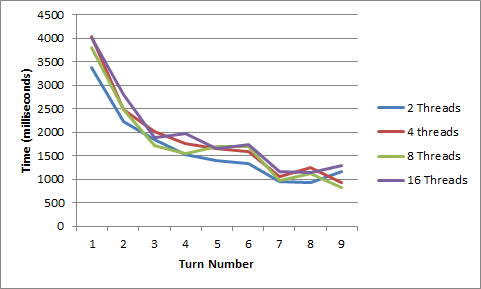
\includegraphics[width=235px]{TimeVsTurn}
\caption{Time per turn}
\centering
\end{figure}

The second chart examines the relationship between the number of nodes that are expanded each turn. If we were to continue this plot over the course of the entire game we would notice that as the available search space reduced, so would the number of expanded nodes.

\begin{figure}[h]
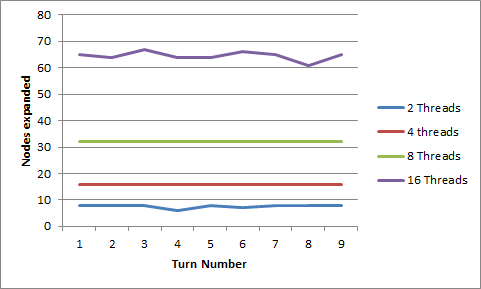
\includegraphics[width=235px]{NodesVsTurn}
\caption{Expanded Nodes per turn}
\end{figure}

We choose not to focus our implementation by optimizing Go heuristic values; instead we only look at the number of captured pieces when determining the static value of the board. Instead we were more interested in improving the speed in which the computer could respond with a valid and hopefully strategic node.

\section{Conclusion}
In the end we were able to successfully complete a parallelized implementation of the Randomized Best-First minimax tree search algorithm that is adapted to the game of Go, something that the creators of the algorithm had not done prior to having their paper published. Unlike the other games where this sort of algorithm accomplished gameplay, Go presents a problem with a significantly larger search space, meaning that we are truly pushing the limits of the computational ability of the algorithm. We were unable to implement the Monte Carlo computer player due to dealing with difficulties imposed by creating our own Java Go game board and efficiently producing one concurrent implementation.\par
Our RBFM implementation indicated that this sort of evaluation is ineffective at producing an artificial player that is proficient at the game of Go. The reason for this is twofold. First is because the algorithm does not look far enough ahead in terms of gameplay to make a move that will subtly lead to a win, since our implementation had a bounded search depth. Our testing indicates that the minimax function assigns heuristic scores to nodes that are too similar to each other to warrant the use of a probability distribution, in other games such as chess, moves from different pieces will lead to much more variance in the minimax score assigned to the root nodes children. Since Go has a uniform play pattern the only time when the RBFM algorithm identifies a node that should be focused upon is when the initial moves leads to predictable play, such as defending a stone that is surrounded on all adjacent intersections by enemy stones except for one space. In this sort of game state it would be more beneficial, on larger game board, to focus our search on other parts of the board where future gameplay could identify a set of plays that force a capture of opponent stones if the opponent predictably plays their stone to capture your piece. The second reason this implementation would not suit playing against human's is the lack of a strong static board position evaluator, but this was by design as we focused on the more on speeding up our implementation.\par
Given additional time we would have liked to optimize our scoring of RBFM nodes in order to take advantage of the probability distributions introduced with the algorithm. This could be done by applying domain-specific knowledge such as the evaluation of groups of stones and the known strategic positioning that is regarded as desirable. Also we would have liked to have been able to implement the other game tree memory management model with master and slave threads as this implementation was spouted to be lock-free. Obviously a concurrently executing Monte Carlo tree search algorithm would have made for a good estimator of the value of our execution times but this model has been accomplished by many others whereas our implementation was novel for this game.


% \appendices
% \section{Challenges}
% \begin{enumerate}
%   \item Implementation of a 2 parallel game trees in Java from pseudo-code.
%   \item Grouping of neighbouring stones on our board for easier position evaluation.
%   \item Determining which parallelized algorithm has the greatest chance to be efficient at a deterministic, zero-sum, combinatorial, perfect information game.
%   \item Getting a minimax algorithm to play efficiently on a game where static evaluation of board position is most of the time useless.
% \end{enumerate}

% \section{Completed Tasks}
% \begin{enumerate}
%   \item Wrote a Randomized Best First Minimax game tree for Go.
%   \item Wrote a Java Go board class which only allows legal moves and provides a score at every stage of the game, which is used as our static position evaluator.
%   \item Located many resources to make sure our implementation is cutting-edge.
% \end{enumerate}

% \section{Remaining Tasks}
% \begin{enumerate}
%   \item Parallelize our implementation of RBFM.
%   \item Writing a Monte-Carlo Tree Search to compare our RBFM implementation to.
%   \item Parallelize our implementation of Monte-Carlo.
%   \item Testing with multiple threads.
%   \item Testing with a 9x9 Go board that is initially empty.
%   \item Testing with a 19x19 Go board that has a specific  set up of initial stones and a correct solution.
%   \item Finishing formalizing our research for the final paper.
% \end{enumerate}

\begin{thebibliography}{1}

\bibitem{RBFM}
Y. Shoham, S. Toledo, \emph{Parallel Randomized Best-First Minimax Search},  Artificial Intelligence 137 (2002) 165--196

\bibitem{Legal}
J. Tromp, G. Farneback, \emph{Combinatorics of Go},
http://tromp.github.io/go/legal.html (2007)

\bibitem{Solutions}
V. Allis, \emph{Searching for Solutions in Games and Artificial Intelligence},
http://fragrieu.free.fr/SearchingForSolutions.pdf (1994)

\bibitem{Remi}
R. Coulom.  \emph{Efficient Selectivity and Backup Operators in Monte-Carlo Tree Search}, 5th International Conference on Computer and Games, May 2006, Turin, Italy. (2006)

\bibitem{PMCTS}
G.M.J-B. Chaslot, J-T. Saito, B. Bouzy, J.W.H.M. Uiterwijk, and H.J. van den
Herik. \emph{Monte-Carlo Strategies for Computer Go} In P.-Y. Schobbens, W. Vanhoof,
and G. Schwanen, editors, Proceedings of the 18th BeNeLux Conference on
Artificial Intelligence, pages 83–90, (2006)

\bibitem{PMCTSB}
G.M.J-B. Chaslot, M.H.M. Winands, and H.J. van den Herik. \emph{Parallel Monte-Carlo Tree Search} 6th International Conference, pages 60-71, (2008)

\end{thebibliography}

\end{document}